\documentclass[ngermn]{book}
\usepackage{style}
\usepackage{figures/tikzpicture}
\usepackage{mathmacros}

\begin{document}
\tableofcontents

\chapter{Deskriptive Statistik}
\chapter{Wahrscheinlichkeitsrechnung und Zufallsvariablen}
	\section{Grundlagen der Wahrscheinlichkeitsrechnung}

In der Wahrscheinlichkeitsrechnung wird die Systematik im Zufall modelliert mit dem Ziel auch zufällige Vorgänge zu quantifizieren, also den Zufall berechenbar zu machen. Wir betrachten Vorgänge, deren Ausgang nicht sicher vorhersehbar ist, eben scheinbar zufällig (stochastisch). Dabei kann es sich durchaus um Vorgänge handeln, die sehr wohl nicht zufällig (deterministisch) sind. Fehlende Informationen oder Kenntnisse der Gesetzmäßigkeiten, nach denen der Vorgang abläuft, lassen eine genaue Vorhersage des Ergebnisses aber nicht zu, weshalb das Ergebnis als Zufallsprodukt angesehen werden muss.

So kann das Werfen eines Würfels als physikalischer Vorgang mit sicherem Ausgang angesehen werden, da bei bekannter Ausgangsposition, Geschwindigkeit und Winkel des Wurfes eine genaue Vorhersage der gewürfelten Zahl möglich wäre. Allerdings fehlen diese Informationen und wir werden das Würfelergebnis vor dem Wurf deshalb als zufällig ansehen. 

Ähnlich sind auch in die Zukunft gerichtete Aussagen (Prognosen) zu einem gewissen Teil immer zufälliger Natur, sofern vollständige Informationen für eine exakte Vorhersage fehlen. Die exakte Prognose des Wirtschaftswachstums beispielsweise ist unmöglich. Daher werden diese Werte auch ständig korrigiert. Das liegt nicht an der Inkompetenz der Experten. Hier werden Modelle genutzt, die das Marktgeschehen so gut wie möglich abbilden. Selbstverständlich sind hier Vereinfachungen unumgänglich, wie bei jedem Modell. Da also nie alle Informationen für die exakte Vorhersage vorliegen, bleibt immer ein unerklärlicher Rest an Unsicherheit, wodurch jede Prognose einen Zufallsfehler enthält.

Diese Unsicherheit wird mit Hilfe der Wahrscheinlichkeitsrechnung modelliert und quantifiziert. Mit Hilfe von Wahrscheinlichkeiten wird ausgedrückt, wie hoch die Chance für das Eintreten eines bestimmten Ergebnisses ist. Je höher  die Wahrscheinlichkeit für einen möglichen Ausgang, desto größer ist die Chance, dass dieser Ausgang tatsächlich beobachtet wird.
 
Diese Vorgänge mit unsicherem Ausgang bezeichnen wir als Zufallsvorgang und unterscheiden zwischen zwei Betrachtungen:
\begin{enumerate}
	\item ex-ante-Betrachtung: Wir betrachten einen Zufallsvorgang (z.B. Würfeln), bevor er abläuft. Dabei ist 
		\begin{itemize}
			\item unbekannt, welches Ergebnis eintreten wird, (welche Zahl fällt wissen wir vorher nicht)
			\item bekannt, welche Ergebnisse potentiell eintreten können (1,2,3,4,5,6) und mit welcher Wahrscheinlichkeit (1/6)
			\item Ziel: 
				\begin{itemize}
					\item Wahrscheinlichkeitsaussagen über mögliche Ereignisse 
					\item Praxisanwendung: Beurteilung von Risiken
				\end{itemize}
		\end{itemize}
	\item ex-post-Betrachtung: Wir betrachten einen Vorgang, nachdem er stattgefunden hat. Dabei ist
		\begin{itemize}
			\item unbekannt, mit welcher Wahrscheinlichkeit ein Ergebnis eintritt - tritt es selten oder eher häufig auf?
			\item bekannt, welches Ergebnis eingetreten ist
			\item Ziel: 
				\begin{itemize}
					\item Von den Beobachtungen wird auf die unbekannte Wahrscheinlichkeit für die Ergebnisse geschlossen 
					\item Praxisanwendung: z.B. Schließen von Häufigkeitsverteilungen in einer Stichprobe auf die Häufigkeitsverteilungen in der Grundgesamtheit
				\end{itemize}
		\end{itemize}
\end{enumerate}

Bewusst möchte ich den Begriff Zufallsexperiment für die Statistikausbildung im Bereich Sozialökonomie nicht verwenden und bevorzuge den Ausdruck Zufallsvorgänge.

	\fbox{\parbox{\textwidth}{
	Ein Zufallsexperiment
		\begin{enumerate}
			\item wird unter kontrollierten Bedingungen nach einer definierten Vorgehensweise ausgeführt,
			\item ist unter gleichen Bedingungen beliebig oft wiederholbar
			\item und hat ein ungewisses Ergebnis, das nicht mit Sicherheit vorhersagbar ist.
		\end{enumerate}	
	}}\\

Nach dieser Vorstellung von einem Zufallsexperiment haben wir es in den Wirtschafts- und Sozialwissenschaften kaum mit Zufallsexperimenten zu tun. Die Datenerhebung erfolgt i.d.R. nicht unter kontrollierten Bedingungen, wie zum Beispiel in der experimentellen Physik möglich. Werden Arbeitslosenzahlen erhoben, lassen sich die Bedingungen nicht kontrollieren, sondern bestenfalls beobachten (Konjunkturlage, BIP, Investitionen, Zinsniveau, usw.). Die Wirtschaftsindikatoren, die vermutlich mit der Arbeitslosenquote zusammenhängen, können nicht vom Forscher als Bestimmungsfaktoren der Arbeitslosenquote vorgegeben werden. Selbstverständlich kann die Arbeitslosenzahl auch nicht ein zweites mal unter den gleichen Bedingungen erhoben werden, da diese sich mit der Zeit - manchmal sogar in kurzer Zeit drastisch - ändern. Selbst das ziehen einer Zufallsstichprobe zur Prognose einer Wählerstimmenverteilung bei der Bundestagswahl (Sonntagsfrage) kann kaum als Zufallsexperiment angesehen werden, da auch hier die Wiederholbarkeit unter gleichen Bedingungen fehlt. Menschen ändern ihre Meinung oder lügen sogar. 

In den Wirtschafts- und Sozialwissenschaften interessieren wir uns oft für  
\begin{itemize}
	\item Stichproben \\Hier sind die relativen Häufigkeiten in der Stichprobe als zufällig anzusehen. Allerdings interessieren wir uns eher für die ex-post-Betrachtung, also wie von der beobachteten Stichprobe auf die Grundgesamtheit geschlossen werden kann. Das ist das Thema der induktiven Statistik, deren Fundament die Wahrscheinlichkeitsrechnung bildet.
	\item Prognosen\\ 
	Welche Ergebnisse oder Ereignisse sind mit einer hohen Wahrscheinlichkeit in Zukunft zu erwarten.
\end{itemize}

%##############################################################################
%##############################################################################
\subsection{Die Definition der Wahrscheinlichkeit}

Die Wahrscheinlichkeitsrechnung ist ein Teilgebiet der reinen Mathematik. Die ersten Statistiker, die sich mit Wahrscheinlichkeiten beschäftigt haben, waren Mathematiker, die sich beim Glücksspiel einen Vorteil verschaffen wollten. Ziel ist es, den Zufall zu modellieren und Gesetzmäßigkeiten oder Muster zu erkennen, so dass die Unsicherheit mit Zahlen beschrieben werden kann.

Der Begriff der Wahrscheinlichkeit wird selbstverständlich im Alltag gebraucht. Die Aussage "Wahrscheinlich wird es morgen regnen." heißt: "Es ist nicht ganz sicher, dass es morgen regnet, aber es sieht ganz danach aus." 
Werden wir gefragt, ob wir zu einer Party kommen werden und wir mit "wahrscheinlich ja" antworten, haben wir die Absicht zu kommen, können es aber nicht garantieren. Der Begriff "wahrscheinlich" drückt aus, dass die Chance, dass wir auf der Party erscheinen werden deutlich höher ist, als dass wir nicht kommen werden. 

Weiterhin haben Wahrscheinlichkeiten im alltäglichen Wortgebrauch die folgenden Eigenschaften:
\begin{enumerate}
	\item Wahrscheinlichkeiten liegen zwischen 0 und 100\%  bzw.  zwischen 0 und 1.
	\item Ist die Wahrscheinlichkeit eines Ereignisses 1 (bzw. 100\%), findet das Ereignis mit Sicherheit statt.
	\item Ist die Wahrscheinlichkeit eines Ereignisses 0, wird das Ereignis auf gar keinen Fall eintreten.
	\item Je größer die Wahrscheinlichkeit eines Ereignisses (z.B. zur Party gehen), desto größer ist die Chance, dass dieses Ereignis eintreten wird.
\end{enumerate}

Diese weithin intuitiv genutzten Eigenschaften finden wir auch in der mathematischen Definition und in den Rechenregeln für Wahrscheinlichkeiten wieder. Auch die Begriffe Ereignis und Ergebnis begegnen uns in der mathematischen Statistik. In den folgenden Abschnitten werden zunächst Grundbegriffe geklärt um mit diesen  das mathematische Modell der Wahrscheinlichkeit zu definieren. In einem weiteren Schritt werden daraus Rechenregeln abgeleitet.
 
 %##############################################################################
%##############################################################################
\subsubsection{Ereignis, Ergebnis, Ereignisraum}
Ergebnisse oder Elementarereignisse sind einzelne mögliche Ausgänge eines zufälligen Vorganges. 
	\begin{itemize}
		\item Werfen einer Münze: Kopf oder Zahl
		\item Werfen eines Würfels: 1,2,3,4,5 oder 6
		\item Leitzins in einem Jahr in Prozent: jede reelle Zahl aus dem Intervall (-100,100)
		\item Geschlecht eines zufällig ausgewählten Menschen: männlich (m) oder weiblich (w)
	\end{itemize}
Die beiden Begriffe Ergebnis und Elementarereignis werden synonym verwendet.

Die Gesamtheit aller Ergebnisse oder Elementarereignisse heißt Ereignisraum. Im mathematischen Sinn ist es eine Menge bezeichnet mit $\Omega$ (gesprochen Omega), deren Elemente die Ergebnisse bzw. Elementarereignisse sind.

\begin{itemize}
		\item Werfen einer Münze: $\Omega = \gkl{Kopf, Zahl}$
		\item Werfen eines Würfels: $\Omega = \gkl{1,2,3,4,5,6}$
		\item  Leitzins in einem Jahr in Prozent:  $\Omega =(-100,100)=\gkl{x| -100 <  x < 100}$
		\item Geschlecht eines zufällig ausgewählten Menschen: $\Omega = \gkl{m, w}$
\end{itemize}

Ereignisse werden gebildet durch das Zusammenfassen von Ergebnissen. Im mathematischen Sinn sind es Teilmengen von $\Omega$. 

\begin{itemize}
		\item Beispiele für Ereignisse beim Würfeln:
			\begin{itemize} 
				\item eine gerade Zahl wird gewürfelt: $\gkl{2,4,6}\subset \gkl{1,2,3,4,5,6}$
				\item höchstens eine 4 wird gewürfelt: $\gkl{1,2,3,4}\subset \gkl{1,2,3,4,5,6}$
				\item mindestens eine 5 wird gewürfelt: $\gkl{5,6}\subset \gkl{1,2,3,4,5,6}$
			\end{itemize}
		\item Beispiele für Ereignisse des Leitzinses in einem Jahr:
			\begin{itemize} 
				\item der Leitzins in einem Jahr ist kleiner als 1\%:  $(-100, 1) \subset (-100, 100)$
				\item der Leitzins in einem Jahr ist mindestens 0,5\%:  $(0,5, 100)  \subset (-100, 100)$
				\item der Leitzins in einem Jahr liegt zwischen -0,1\% und +0,1\%: $(-0,1, 0,1)  \subset (-100, 100)$
			\end{itemize}
\end{itemize}

Ereignisse sind auch 
\begin{itemize}
	\item die Elementarereignisse - also Ereignisse mit nur einem Element,
	\item der gesamte Ereignisraum $\Omega$,
	\item und die leere Menge - in Zeichen $\gkl{}$ oder $\emptyset$.
\end{itemize}

Alle möglichen Ereignisse beim Würfeln sind demnach

\begin{tabular}{ccccccc}\\\hline
$\gkl{}$&$\gkl{1}$& $\gkl{1,2}$ & $\gkl{1,2,3}$ & $\gkl{1,2,3,4}$ &  $\gkl{1,2,3,4,5}$ & $\gkl{1,2,3,4,5,6}=\Omega$\\
	 &$\gkl{2}$ & $\gkl{1,3}$& $\gkl{1,2,4}$& $\gkl{1,2,3,5}$& $\gkl{1,2,3,4,6}$ &\\
	 &$\gkl{3}$ & $\gkl{1,4}$& $\gkl{1,2,5}$& $\gkl{1,2,3,6}$& $\gkl{1,2,3,5,6}$&\\
	 &$\gkl{4}$ & $\gkl{1,5}$& $\gkl{1,2,6}$& $\gkl{1,2,4,5}$& $\gkl{1,2,4,5,6}$&\\
	 &$\gkl{5}$ & $\gkl{1,6}$ & $\gkl{1,3,4}$& $\gkl{1,2,4,6}$& $\gkl{1,3,4,5,6}$&\\ 
	 &$\gkl{6}$ & $\gkl{2,3}$& $\gkl{1,3,5}$& $\gkl{1,2,5,6}$& $\gkl{2,3,4,5,6}$&\\
	 &		 & $\gkl{2,4}$& $\gkl{1,3,6}$& $\gkl{1,3,4,5}$& &\\
	 &		 & $\gkl{2,5}$& $\gkl{1,4,5}$& $\gkl{1,3,4,6}$& &\\
	 &		 & $\gkl{2,6}$& $\gkl{1,4,6}$& $\gkl{1,3,5,6}$ & &\\
	 &		 & $\gkl{3,4}$& $\gkl{1,5,6}$& $\gkl{1,4,5,6}$& &\\ 
	  &		 & $\gkl{3,5}$& 			&$\gkl{2,3,4,5}$ & &\\
	 &		 & $\gkl{3,6}$& 			&$\gkl{2,3,4,6}$ & &\\
	 &		&  $\gkl{4,5}$& 			&$\gkl{2,3,5,6}$ & &\\
	 &		& $\gkl{4,6}$ & 			&$\gkl{2,4,5,6}$ & &\\
	 & 		& $\gkl{5,6}$& 			&$\gkl{3,4,5,6}$& &\\
	 \hline
\end{tabular}
\\

HINWEIS: Ereignisse sind Teilmengen und demzufolge haben sie auch die Eigenschaften von Mengen:
\begin{itemize}
	\item In einem Ereignis existiert jedes Element nur einmal, also ist z.B. $\gkl{1,2,4,5,5}$ kein Ereignis sondern $\gkl{1,2,4,5}$.
	\item Die Reihenfolge der Elemente ist irrelevant, also sind z.B. die Ereignisse $\gkl{1,2,4,5}$ und $\gkl{2,1,4,5}$ und $\gkl{4,1,2,5}$ identisch.
\end{itemize}

Betrachten wir das Ereignis \emph{eine gerade Zahl wird gewürfelt}. Mathematisch ausgedrückt handelt es sich also um die Menge $$A=\gkl{2,4,6}.$$ Wird nun z.B. eine 4 gewürfelt, dann sagen wir \emph{das Ereignis A ist eingetreten}. Die gewürfelte Zahl muss also ein Element aus A sein, damit A eintritt. 

Wird eine ungerade Zahl gewürfelt - z.B. eine 5 - dann ist A nicht eingetreten. 
\begin{center}
	\textbf{ Welche der oben aufgelisteten Ereignisse ist eingetreten, wenn eine 5 gewürfelt wird?}
\end{center}


Allgemein: Ein Ereignis A tritt ein, wenn der Ausgang des Zufallsvorganges ein Element aus A ist. Das Ereignis A tritt nicht ein, wenn der Ausgang des Zufallsvorganges kein Element aus A ist.

\subsubsection{Das Ereignis $\overline{A}$ - \emph{nicht A}}

Das Ereignis \emph{nicht A} tritt genau dann ein, wenn A nicht eingetreten ist. Wir sprechen auch vom komplementären Ereignis zu A oder vom Komplement zu A. Weiterhin wird $\overline{A}$ auch als Gegenereignis zu A bezeichnet.

Um das Ereignis zu erzeugen, entfernen wir aus dem Ereignisraum $\Omega$ alle Elemente aus A. Damit erhalten wir die Menge mit allen Elementen aus $\Omega$, die nicht in A enthalten sind. 

Würfel-Beispiel: Sei $$A = \gkl{2,4,6},$$ 
also eine gerade Zahl wird gewürfelt. Dann wird $\overline{A}$ gebildet, indem aus $\Omega = \gkl{1,2,3,4,5,6}$ die Elemente 2,4 und 6 entfernt werden, also
 $$\overline{A}=\gkl{1,3,5}.$$
Das komplementäre Ereignis zu \emph{eine gerade Zahl wird gewürfelt} ist \emph{eine ungerade Zahl wird gewürfelt}. 

Das Komplement zu $\Omega$ ist demnach die leere Menge $\emptyset$.

\subsubsection{Das Ereignis $A \cap B$ - \emph{A und B}}

Das Ereignis  \emph{A und B} tritt genau dann ein, wenn A und B gleichzeitig eintreten. 

Diese Menge beinhaltet die Elemente, die sowohl in A als auch in B enthalten sind. Wir sprechen auch vom Schnitt, Durchschnitt oder Schnittmenge der beiden Mengen und sprechen: A geschnitten B. 

Würfel-Beispiel:
 
Das Ereignis $B=\gkl{1,2,3,4}$ ist \emph{höchstens eine 4 wird gewürfelt}. Das Ereignis $A\cap B$ ist, eine \emph{gerade Zahl höchstens 4} wird gewürfelt. Dieses Ereignis wird gebildet, indem wir die Elemente in A daraufhin überprüfen, ob sie auch in B enthalten sind. Nur diese gehören dann in die Schnittmenge
$$A\cap B = \gkl{\textbf{2},\textbf{4},6}\cap \gkl{1,\textbf{2},3,\textbf{4}} = \gkl{2,4}.$$

Würfeln wir eine 2 (oder 4), tritt nicht nur A ein sondern auch B - eben \emph{A und B}.

\subsubsection{Disjunkte Ereignisse}

Zwei Ereignisse A und B heißen disjunkt, wenn sie kein gemeinsames Element haben. Diese Ereignisse können dann nicht zusammen eintreten. Die Schnittmenge ist dementsprechend die leere Menge, also $$A\cap B = \emptyset.$$

Würfel-Beispiel: Sei $A=\gkl{2,4,6}\ \text{und}\  C=\gkl{1,3}$. Offensichtlich gibt es in A kein Element, dass auch in C enthalten ist, also gilt

$$A\cap C = \gkl{2,4,6}\cap \gkl{1,3} = \emptyset.$$ A und C heißen disjunkt. Das heißt, dass A und C nicht gemeinsam eintreten können. Da in C nur ungerade Zahlen enthalten sind, kann C mit dem Ereignis \emph{eine gerade Zahl wird gewürfelt} nicht gleichzeitig eintreten. Das Eintreten von A schließt C aus und umgekehrt.

Beispiel Komplementäre Ereignisse: Komplementäre Ereignisse sind immer disjunkt, denn in \emph{nicht A} ($\overline{A}$) sind definitionsgemäß keine Elemente aus A enthalten. Demnach gilt für komplementäre Ereignisse immer
$$A\cap \overline{A} = \emptyset$$

ACHTUNG: Komplementäre Ereignisse sind zwar immer disjunkt, aber nicht immer sind disjunkte Ereignisse komplementär. Bei komplementären Ereignissen tritt immer eins der beiden Ereignisse ein - das Eintreten des einen hat das Nicht-Eintreten des anderen zur Folge. Sind zwei Ereignisse disjunkt, aber nicht komplementär, können auch beide nicht eintreten. 
Betrachten wir nochmal das Würfelbeispiel mit den disjunkten Ereignissen A und C. Im Fall einer gewürfelten 5 treten beide nicht ein, weshalb es sich auch nicht um komplementäre Ereignisse handelt.

\subsubsection{Das Ereignis $A\cup B$ - \emph{A oder B}}
Das Ergeignis \emph{A oder B} tritt genau dann ein, wenn entweder A oder B oder beide eingetreten sind. Mit dem Eintreten von A ist auch $A\cup B$ eingetreten - das gleiche gilt für B. 

Das Ereignis beinhaltet alle Elemente, die in A enthalten sind und alle Elemente aus B. 

ACHTUNG: Das Ereignis  \emph{A oder B} wird oft mit \emph{A und B} ($A\cap B$) verwechselt, da hier eben alle Elemente von A und B enthalten sind. 
Die Formulierung \emph{A oder B} bezieht sich aber auf das Kriterium, wann das Ereignis eintritt, 
$$\text{nämlich wenn A oder B eintritt}$$
und nicht darauf, wie die Menge gebildet wird,
 $$\text{nämlich durch die Vereinigung aller Elemente aus A und B}.$$

Würfel-Beispiel:

Sei $A = \gkl{2,4,6}$ und $B=\gkl{1,2,3,4}$. Das Ereignis \emph{A oder B} bedeutet, dass entweder eine gerade Zahl oder eine Zahl höchstens 4 oder auch beides - eine gerade Zahl höchstens 4 - gewürfelt wird. Das Ereignis enthält die geraden Zahlen und die Zahlen, die höchstens 4 sind 
$$A\cup B = \gkl{2,4,6} \cup \gkl{1,2,3,4}= \gkl{1,2,3,4,6}.$$

Anmerkung zu den komplementären Ereignissen

Bei komplementären Ereignissen $A, \overline{A}$ tritt immer eins der beiden Ereignisse ein - das Eintreten des einen hat das Nicht-Eintreten des anderen zur Folge. Das Ereignis \emph{A oder nicht A} tritt mit Sicherheit ein $$A \cup \overline{A} = \Omega.$$

Hier liegt der Unterschied zu disjunkten Ereignissen, die keine Komplementäre sind. Die können auch beide nicht eintreten. 
Betrachten wir nochmal das Würfelbeispiel mit den disjunkten Ereignissen A und C, die nicht komplementär sind. Im Fall einer gewürfelten 5 treten beide nicht ein.



\begin{center}
\begin{tabular}{|c|c|}\hline
	komplementäre Ereignisse & disjunkte Ereignisse,\\ 
	 & die nicht komplementär sind \\ \hline
	A, $\overline A$ & A, B\\
	$A\cap \overline{A} = \emptyset$ & 	$A\cap B = \emptyset$ \\
	$A\cup \overline{A} =\Omega$ & $A\cup B \neq\Omega$\\\hline
\end{tabular}
\end{center}

\subsubsection{Axiome von Kolmogoroff}

Die Wahrscheinlichkeit (P) gibt als Wert an, wie groß die Chance ist, dass ein gewisses Ereignis (A) eintritt. Den Ereignissen A wird eine Wahrscheinlichkeit P(A) zugeordnet. Die Wahrscheinlichkeit ist also eine Abbildung der Teilmengen aus $\Omega$ - also der Ereignisse - auf die reellen Zahlen
$$A \rightarrow P(A)\in \R$$
und wird genau genommen als Wahrscheinlichkeitsmaß definiert.

Die Wahrscheinlichkeit im mathematischen Sinn wird nicht hergeleitet, abgeleitet oder bewiesen. Es ist ein Modell zur Messung von Unsicherheit, das axiomatisch aufgestellt wird, d.h. es wurden sinnvolle und zweckmäßige Festlegungen getroffen, die die Eigenschaften von Wahrscheinlichkeiten implizieren.


	\fbox{\parbox{\textwidth}{
	Axiome von Kolmogoroff:
	\begin{enumerate}
		\item P($\Omega$)=1
		\item $P(A)>0$, falls $A\neq\emptyset$
		\item $P(A\cup B) = P(A) + P(B)$ falls $A\cap B =\emptyset$
	\end{enumerate}
	}}\\

Das erste Axiom besagt, dass das sichere Ereignis $\Omega$ - also das mit Sicherheit auftretende Ereignis - die Wahrscheinlichkeit 1 hat. 

Das zweite Axiom besagt, dass ein Ereignis eine positive Wahrscheinlichkeit hat, wenn es sich nicht um das unmögliche Ereignis handelt.
 
Das dritte Axiom besagt, dass die Wahrscheinlichkeit des Ereignisses \emph{A oder B} als Summe der Einzelwahrscheinlichkeiten von A und B berechnet werden kann, vorausgesetzt A und B sind disjunkt. Hier handelt es sich also in gewisser Weise um eine Rechenregel.

Was nicht axiomatisch festgelegt ist, aber als Eigenschaften von Wahrscheinlichkeiten gilt, ist 
\begin{enumerate}
    \item dass Wahrscheinlichkeiten nicht größer als 1 werden.
    $$P(A)\leq 1$$
    \item dass die Wahrscheinlichkeit vom unmöglichen Ereignis ist 0.
    $$P(\emptyset)=0$$
\end{enumerate}

Tatsächlich implizieren die Axiome von Kolmogoroff diese Eigenschaften, d.h. diese Eigenschaften können aus den Axiomen von Kolmogoroff hergeleitet werden.

\begin{enumerate}
    \item Wahrscheinlichkeiten sind nicht negativ.
    \item Wahrscheinlichkeiten werden nicht größer als 1.
    \item Die Wahrscheinlichkeit vom unmöglichen Ereignis ist 0.
\end{enumerate}

Würfel-Beispiel:



%####################################################################################
%####################################################################################
%####################################################################################
%	\graphicspath{{./Bilder/}}
%		\begin{center}
%			\fbox{\scalebox{0.35}[0.3]
%			{\includegraphics{Didaktik2.pdf}}}
%		\end{center}
%####################################################################################
%####################################################################################
%####################################################################################
	\section{Zufallsvariablen}
%\listoftodos

\begin{bsp}
		$1$ mal würfeln. \\

		$\begin{aligned}
			 \underset{(Omega)}{\Omega} &= \text{ Menge der möglichen Ausgänge} \\
																	&= \text{ Ergebnisse } 
		\end{aligned}$

\hfill
		\begin{tikzpicture}[scale=0.7,baseline={(current bounding box.center)}]
		%	\draw[help lines] (0,0) grid (8,5);
			\draw (2,0) -- (2,5) -- (8,5) -- (8,0) -- (2,0);
			\node[rotate=0] at (3,4) {\LARGE 1};
			\node[rotate=10] at (4,3) {\LARGE 2};
			\node[rotate=-0] at (5,4) {\LARGE 3};
			\node[rotate=-0] at (6.1,2.3) {\LARGE 4};
			\node[rotate=-20] at (4.3,1.5) {\LARGE 5};
			\node[rotate=0] at (5.2,1) {\LARGE 6};
			\draw [->] (2,2.3) -- (0,2.3);
		\end{tikzpicture}
%
\vspace{-0.01\textheight}
	\begin{itemize}[]
		\item% 
			\begin{flalign*}
			P(A) & = P (\text{gerade Zahlen})  \\
					 & = P(\hspace{-1.0em} \underbrace{ \set{2,4,6} }
							_{\substack{\text{Anzahl der } \\ \text{günstigen Erg.}}} \hspace{-1.0em}) 
						 = \frac{\text{Anzahl der günstigen Ergebnisse}}
							{\underbrace{\text{Anzahl der möglichen Ergebnisse}}_
							{\substack{= \text{Anzahl d. Elemente in } \Omega}}} 
						 = \frac{3}{6}\\
					 &\\
			 P (\set{1}) &= \frac{1}{6}\\ 
			\end{flalign*}	
	\end{itemize}

\begin{minipage}{0.4\linewidth}
	\begin{tikzpicture}[scale=0.7]
		%\draw[help lines] (0,0) grid (8,5);
		% Box mit Omega
		\draw (2,0.5) -- (2,4.5) -- (7.5,4.5) -- (7.5,0.5) -- (2,0.5);
		\node at (1,4.5) {\Huge $\Omega$};
		% Zahlen in der Box
		\foreach \x/\y/\n/\r in {2.7/3.5/1/0,2.9/1.8/2/5,4.7/3.5/3/7,4.7/1.2/4/-5,6.7/3.5/5/0,6.9/1.5/6/0}
		\node[rotate=\r] at (\x,\y) {\LARGE \n};
		% Zahlen ausserhalb der Box
		\foreach \x/\y/\n/\r in {2.7/3.5/1/0,2.9/1.8/2/5,4.7/3.5/3/7,4.7/1.2/4/-5,6.7/3.5/5/0,6.9/1.5/6/0}
		\ifthenelse{\equal{\n}{1} \OR \equal{\n}{3} \OR \equal{\n}{5}}%
			{\node at (\x+0.4,\y+1.6) {\LARGE \n}}%
			{\node at (\x+0.1,-0.5) {\LARGE \n}};
		% Zeichnet die Pfeile
		\foreach \x/\y/\n/\r in {2.7/3.5/1/0,2.9/1.8/2/5,4.7/3.5/3/7,4.7/1.2/4/-5,6.7/3.5/5/0,6.9/1.5/6/0}
		\ifthenelse{\equal{\n}{1} \OR \equal{\n}{3} \OR \equal{\n}{5}}%
			{\draw[thick,->] (\x,\y+0.5) -- (\x+0.34,\y+1.2)}%
			{\draw[thick,->] (\x,\y-0.5) -- (\x+0.1,-0.1)};
	\end{tikzpicture}
\end{minipage}
%
\begin{minipage}{0.6\linewidth}
	ZV $X = $ Augenzahl\\
	Wahrscheinlichkeitsverteilung
	\def \var {0.10\linewidth}
	\begin{tabular}{m{0.28\linewidth}|m{\var} m{\var}m{\var}m{\var}m{\var}m{\var}}
		\centering $x_i$  & 1 & 2 & 3 & 4 & 5 & 6 \tabularnewline
		\hline
		\centering $P(X = x_i)$ & $\frac{1}{6}$ & $\frac{1}{6}$ & $\frac{1}{6}$ 
														& $\frac{1}{6}$ & $\frac{1}{6}$ & $\frac{1}{6}$ 	
	\label{Wahrscheinlichkeitsverteilung}
	\end{tabular}
\end{minipage}
~\\	
\begin{minipage}{0.45\linewidth}
	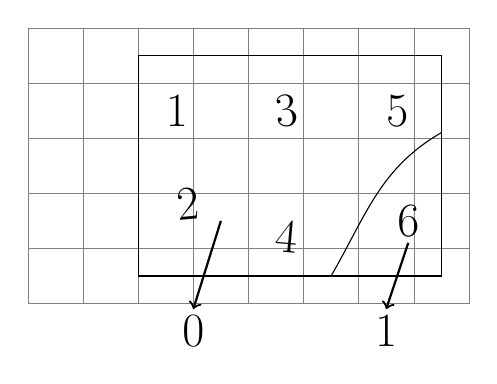
\begin{tikzpicture}[scale=0.7]
		\draw[help lines] (0,0) grid (8,5);
		% Box mit Omega
		\draw (2,0.5) -- (2,4.5) -- (7.5,4.5) -- (7.5,0.5) -- (2,0.5);
		% Zahlen in der Box
		\foreach \x/\y/\n/\r in {2.7/3.5/1/0,2.9/1.8/2/5,4.7/3.5/3/7,4.7/1.2/4/-5,6.7/3.5/5/0,6.9/1.5/6/0}
		\node[rotate=\r] at (\x,\y) {\LARGE \n};
		% Schrägstrich in der Box 
		\draw (5.5,0.5) to [out=60,in=-150] (7.5,3.1);
		% Pfeile an den Unterteilung : 0
			%definiere (lokale Variabeln)
			\def \x {3} 
			\def \y {-0.1}
		\draw[thick,->] (\x+0.5,1.5) -- (\x,\y);
		\node at (\x,\y-0.4) {\LARGE 0};
		% Pfeile an den Unterteilung : 1
			%definiere (lokale Variabeln)
			\def \x {6.5} 
			\def \y {-0.1}
		\draw[thick,->] (\x+0.4,1.1) -- (\x,\y);
		\node at (\x,\y-0.4) {\LARGE 1};
	\end{tikzpicture}
\end{minipage}
%
\begin{minipage}{0.55\linewidth}
	ZV $Y$ gibt an, ob eine $6$ gewürfelt wurde:
		\begin{itemize}[]
			\item $y_1 = 0 :$ keine $6$ wurde gewürfelt
			\item $y_2 = 1 :$ eine 6 wurde gewürfelt
		\end{itemize}
	Wahrscheinlichkeitsverteilung\\
	\begin{tabular}{c | c c}
		$y_i$ & 0 & 1\\
		\hline
		\vspace{1em} $ P( y = y_1)$ & $\frac{5}{6}$ & $\frac{1}{6}$
	\end{tabular}
\end{minipage}

\begin{minipage}{0.45\linewidth}
	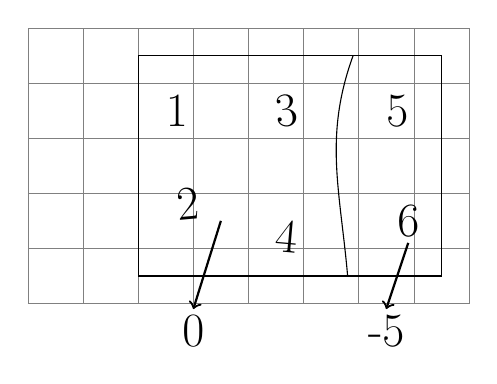
\begin{tikzpicture}[scale=0.7]
		\draw[help lines] (0,0) grid (8,5);
		% Box mit Omega
		\draw (2,0.5) -- (2,4.5) -- (7.5,4.5) -- (7.5,0.5) -- (2,0.5);
		% Zahlen in der Box
		\foreach \x/\y/\n/\r in {2.7/3.5/1/0,2.9/1.8/2/5,4.7/3.5/3/7,4.7/1.2/4/-5,6.7/3.5/5/0,6.9/1.5/6/0}
		\node[rotate=\r] at (\x,\y) {\LARGE \n};
		% Schrägstrich in der Box 
		\draw (5.8,0.5) to [out=95,in=250] (5.9,4.5);
		% Pfeile an den Unterteilung : 0
			%definiere (lokale Variabeln)
			\def \x {3} 
			\def \y {-0.1}
		\draw[thick,->] (\x+0.5,1.5) -- (\x,\y);
		\node at (\x,\y-0.4) {\LARGE 0};
		% Pfeile an den Unterteilung : 1
			%definiere (lokale Variabeln)
			\def \x {6.5} 
			\def \y {-0.1}
		\draw[thick,->] (\x+0.4,1.1) -- (\x,\y);
		\node at (\x,\y-0.4) {\LARGE -5};
	\end{tikzpicture}
\end{minipage}
%
\begin{minipage}{0.55\linewidth}
	\underline{Gewinnspiel:}
		\begin{itemize}
			\item bei $5,6 \to$ Verlust von $5EURO$
			\item bei $1,2,3$ oder $4$ Gewinn in Höhe der doppelten Augenzahl 
		\end{itemize}
\end{minipage}

	ZV $Z =$ Gewinn / Verlust in EURO mit 
	Realisationsmöglichkeiten: $-5,2,4,6,8$\\

\begin{minipage}{0.45\linewidth}
\begin{tikz}[scale=0.5]
	\draw[help lines] (0,0) grid (8,5);	
\end{tikz}
\end{minipage}
\begin{minipage}{0.55\linewidth}
	\underline{Wahrscheinlichkeitsverteilung von $Z$}
	\begin{tabular}{c | c c c c c}
		$Z_i$ 	&  -5		& 	2		&		4		& 	6		&		8		\\
		\hline
		\vspace{1em} $ P( Z = z_1)$ & $\frac{2}{6}$ & $\frac{1}{6}$ & $\frac{1}{6}$ & $\frac{1}{6}$ & $\frac{1}{6}$ 
	\end{tabular}
\end{minipage}

\begin{minipage}{0.45\linewidth}
\begin{tikz}[scale=0.5]
	\draw[help lines] (0,0) grid (8,5);	
\end{tikz}
\end{minipage}
\begin{minipage}{0.55\linewidth}
	\underline{Verteilungsfunktion von $Z$}: $F(z) = P(Z \leq z), z\in \R$
	\begin{tabular}{c | c c c c c}
		$Z_i$ 	&  -5		& 	2		&		4		& 	6		&		8		\\
		\hline
		\vspace{1em} $ P( Z \leq z_1)$ & $\frac{2}{6}$ & $\frac{3}{6}$ & $\frac{4}{6}$ & $\frac{5}{6}$ & $\frac{6}{6}=1$ 
	\end{tabular}
\end{minipage}
~\\
$\begin{aligned}
	E(Z)	&= z_1 \cdot \underbrace{P(Z=z_1)}_{p_1} + z_2 \cdot \underbrace{P(Z=z_2)}_{p_2}
						+ \cdot + z_5 \cdot \underbrace{P(Z=z_5)}_{p_5}\\
				&= z_1 p_1 + z_2 p_2 + \dots + z_5 p_5\\
				&= -5 \cdot \frac{2}{6} + 2 \cdot \frac{1}{6} + 4 \cdot \frac{1}{6}
				+ 6 \cdot \frac{1}{6}	+ 8\cdot \frac{1}{6}\\
				&= + \underline{\underline{1,\ov{6}}}
\end{aligned}$
\begin{tabbing}
	\underline{Interpretation:} \= Spielen wir dieses Spiel sehr oft, wird der 
		Gewinn im Durchschnitt bei $1,67$EURO liegen.
\end{tabbing}
\end{bsp}

\underline{deskriptiv}: Varianz und Standardabweichung \\
Varianz \dots mittlere quadrierte Abweichung von arithmetischen Mittel
	$$ \sum (\alpha_i - \ov{x})^2 h_i = s_x^2$$
$\alpha_i$ $\leftrightarrow$ Realisationsmöglichkeiten $x_i$ \\
$\ov{x}$ $\leftrightarrow$ $E(X)$	\\
$h_i$ $\leftrightarrow$ $p_i$

\underline{Varianz einer ZV $X$}: 
	$Var(X) = \sigma^2 = \sum_{i=1}^{k}(x_i - E(X))^2 p_i		
		= E((X-E(X))^2)$, wobei $p_i = P(X=x_i)$\\
Erwartungswert der quadrierten Differenzen für viele Versuchswiederholungen gilt  

\begin{tabular}{p{0.5\linewidth} p{0.5\linewidth}}
\hfill 23 & 23 \hfill\\
\end{tabular}

%%%%%%%%%%%%%%%%%%%%%%%%%%%%%%%%%%%%%%%%%%%%%%%%%%%%%%%%%
\def\varA{\mbox{
	\begin{tabular}{@{}l@{}}
		berechnet mit Realisations-\\möglichkeiten und $p_i$
	\end{tabular}
	}
	\hspace{0em}
}
\def\varB{\mbox{
	\begin{tabular}{@{}l@{}}
		berechnet mit Realisationen bzw.\\ Beobachtungen und $h_i$
	\end{tabular}
	}
	\hspace{0em}
}
%%%%%%%%%%%%%%%%%%%%%%%%%%%%%%%%%%%%%%%%%%%%%%%%%%%%%%%%%

	$$ \underbrace{Var(X)}_{\varA} \approx \; \underbrace{s_x^2}_{\varB}$$

%\begin{tabular}{p{0.15\linewidth} | p{0.1\linewidth} | p{0.1\linewidth} | p{0.1\linewidth} | p{0.1\linewidth} | p{0.1\linewidth}}
\begin{tabular}{c | c | c | c | c | c l }
$z_i$	  & -5 & 2 & 4 & 6 & 8\\
\hline   
$p_i$  &  $\frac{2}{6}$  & $\frac{1}{6}$ & $\frac{1}{6}$ & $\frac{1}{6}$ & $\frac{1}{6}$ \\
$(z_i -1,\ov{6})^2$ & 44,44 & 0,11 & 5,44 & 18,78 & 40,11 \\
$(z_i -1,\ov{6})^2$ & 14,81 & 0,018 & 0,91 & 3,13 & 6,685 \\
\end{tabular}
\begin{tabular}{l}
\\ \\ \\
$\Sigma = \underline{\underline{25,55}}$	
\end{tabular}

$Var(Z) = \sigma_Z^2 = 25,55$\\
Standardabweichung: $\sigma_Z = \sqrt{Var(Z)} = \sqrt{25,55} = $ \underline{\underline{5,05}} \\

Im Mittel weichen die Realisationen von $Z$ (also der Gewinn) um 5,05 EURO von durchschnittlichen bzw. erwarteten Gewinn 1,67 EURO ab.\\

$ZV$ $Y$ sei auch ein Gewinn in einem Glückspiel

\begin{tabular}{c | c c c c}
	$y_i$		&		0		&		1		&		5		&		10	\\
	\hline
	$p_i$		&	0,35	& 0,5		&		0,1	&	0,05  \\
	$(y_i -\underbrace{E(Y))}_{= 1,5}^2$
					&	2,25	&	0,25	&	12,15	&	72,25
\end{tabular}

$\begin{aligned}
	E(Y) &= 0,35 \dot 0 + 0,5 \cdot 1 + 0,1 \cdot 5 + 0,05 \cdot 10 =
	\underline{\underline{1,5}} EURO \\
%
	E(Z) &= +1,67  EURO \\
%
	Var(Y) &= 2,25 \cdot 0,35 + 0,25 \cdot 0,5 + 12,25 \cdot 0,1 +
	72,26 \cdot 0,05 \\
	&= \text{\underline{\underline{5,75}}} = \sigma_y^2\\
%
	\sigma_y &= \sqrt{5,75} = \underline{\underline{2,4}} \\
%
	\sigma_z &= \underline{\underline{5,05}} \\
\end{aligned}$

$$\begin{aligned}
	E(Y)		 &<	E(Z) \\
	\sigma_Y &< \sigma_Z
\end{aligned}$$

Summe von zwei Würfeln $ = X$

$\begin{aligned}
\Omega = \{& \overbrace{(1,1)}^{X=2}, \overbrace{(1,2)}^{X=3}, \dots , 
	\overbrace{(1,6)}^{X=7} \\
					 & \underbrace{(2,1)}_{X=3}, \underbrace{(2,2)}_{X=4}, 
	\underbrace{(2,6)}_{X=8} \\
	 				 & \underbrace{(6,1)}_{X=7}, \underbrace{(6,2)}_{X=8}, \dots ,
	\underbrace{(6,6)}_{X=12}\} \quad \text{mögliche Ergebnisse}
\end{aligned}$
\par
alle Ergebnisse haben die gleiche W. \\
6x6 mögliche Ergebnisse = Anzahl der möglichen Ergebnisse

$\begin{aligned}
\text{z.B.} \quad & P(X = 3) = P(\set{(1,2), (2,1)}) = \frac{2}{36}\\
						& P(X = 7) = \frac{6}{36} = \frac{1}{6}
\end{aligned}$

$(1,6) , (6,1)$\\
$(2,5), (5,2) $\\
$(3,4), (4,3)$ \\

\begin{tabular}{c | c | c}
$x_i$	&	$p_i$	&	$P(X \le x_i)$ \\
\hline
	2		&	1/36	&			1/36			\\
	3		&	2/36	&			3/36			\\	
	4		&	3/36	&			6/36			\\	
	5		&	4/36	&		 10/36			\\	
	6		&	5/36	&		 15/36			\\	
	7		&	6/36	&		 21/36			\\	
	8		&	5/36	&		 26/36			\\	
	9		&	4/36	&		 30/36			\\	
	10	&	3/36	&		 33/36			\\	
	11	&	2/36	&		 35/36			\\	
	12	&	1/36	&		  1/36			\\	
\end{tabular}

$\begin{aligned}
	P(X \leq 7) &= \frac{21}{36} \\
	P(X \geq 7) &= P(X > 6) = 1 - P(\leq 6) =  21/36 \\
	P(X < 7) &= P(X \leq 6) = \frac{15}{36} \\
	P(X > 7) &= 1 - P(X \leq 7) = \frac{15}{36} \\
	\\
	P(5 < X \leq 10) &= 
\end{aligned}$
 %Dennis 
\chapter{Induktive Statistik}
%
% Erstellt einen Eintrag "Index" ins Inhaltsverzeichnis
%
\cleardoublepage
\addcontentsline{toc}{chapter}{Index}
\printindex

\end{document}
